% 
% Lecture Template for ME3050 -  Dynamics Modeling and Controls - Tennessee Technological University
%
% Tristan Hill, May 07, 2020 - June 12, 2020, % Spring 2020 - Summer 2020
% Module 7 - Damping Elements
% Topic 2 - Mechanical Damping
%

\documentclass[fleqn]{beamer}                         % for presentation (has nav buttons at bottom)
%\documentclass[handout]{beamer}  % for handout 
\usepackage{beamerthemesplit}
\usepackage{amsmath}
\usepackage{listings}
\usepackage{multicol}
\usepackage{framed}

\usepackage{amsmath}
\usepackage{bm}

\beamertemplateballitem

% custom colors
\definecolor{TTUpurple}{rgb}{0.3098, 0.1607, 0.5176} % TTU Purple (primary)
\definecolor{TTUgold}{rgb}{1.0000, 0.8666, 0.0000} % TTU Gold (primary) 
\definecolor{mygray}{rgb}{.6, .6, .6}
\definecolor{mypurple}{rgb}{0.6,0.1961,0.8}
\definecolor{mybrown}{rgb}{0.5451,0.2706,0.0745}
\definecolor{mygreen}{rgb}{0, .39, 0}
\definecolor{mypink}{rgb}{0.9960, 0, 0.9960}

% color commands
\newcommand{\R}{\color{red}}
\newcommand{\B}{\color{blue}}
\newcommand{\BR}{\color{mybrown}}
\newcommand{\K}{\color{black}}
\newcommand{\G}{\color{mygreen}}
\newcommand{\PR}{\color{mypurple}}
\newcommand{\PN}{\color{mypink}}
\newcommand{\OR}{\color{TTU}}
\newcommand{\GD}{\color{TTUgold}}

% beamer colors
\setbeamercolor{palette primary}{bg=TTUpurple,fg=TTUgold}
\setbeamercolor{palette secondary}{bg=black,fg=TTUgold}
\setbeamercolor{palette tertiary}{bg=black,fg=TTUpurple}
\setbeamercolor{palette quaternary}{bg=TTUgold,fg=black}
\setbeamercolor{structure}{fg=TTUpurple} % itemize, enumerate, etc
\setbeamercolor{section in toc}{fg=TTUpurple} % TOC sections


\newcommand{\Lagr}{\mathcal{L}} % lagrangian

\newcommand{\hspcu}{\underline{\hspace{20mm}}} % large horizontal space w underline
\newcommand{\vspccc}{\vspace{6mm}\\} % large vertical space
\newcommand{\vspcc}{\vspace{4mm}\\}   % medium vertical space
\newcommand{\vspc}{\vspace{2mm}\\}     % small vertical space

\newcommand{\hspcccc}{\hspace{10mm}} % large horizontal space
\newcommand{\hspccc}{\hspace{6mm}} % large horizontal space
\newcommand{\hspcc}{\hspace{4mm}}   % medium horizontal space
\newcommand{\hspc}{\hspace{2mm}}     % small horizontal space

\newsavebox{\mybox} % custom box


\newcommand{\MNUM}{7\hspace{2mm}} % Module number
\newcommand{\TNUM}{2\hspace{2mm}} % Topic number 
\newcommand{\moduletitle}{Damping Elements} % Titles and Stuff
\newcommand{\topictitle}{Mechanical Damping} 

\newcommand{\sectiontitleI}{A Better Model} % More Titles and Stuff
\newcommand{\sectiontitleII}{Oscillation and Decay}
\newcommand{\sectiontitleIII}{Sources of Damping}
\newcommand{\sectiontitleIV}{Dampers Damp!}

\author{ME3050 - Dynamics Modeling and Controls}
\title{Lecture Module - \moduletitle}
\date{Mechanical Engineering\vspc Tennessee Technological University}

\begin{document}

\lstset{language=MATLAB,basicstyle=\ttfamily\small,showstringspaces=false}

\frame{\titlepage \center\begin{framed}\Large \textbf{Topic \TNUM - \topictitle}\end{framed} \vspace{5mm}}

% Section 0 - Outline
\frame{
	
	\large \textbf{Topic \TNUM - \topictitle} \vspace{3mm}\\
	
	\begin{itemize}
	
		\item \sectiontitleI    \vspc % Section I
		\item \sectiontitleII 	\vspc % Section II
		\item \sectiontitleIII 	\vspc %Section III
		\item \sectiontitleIV 	\vspc %Section IV
	
	\end{itemize}

}

% Section I
\section{\sectiontitleI}

	% Section I - Frame I
	\frame{ \small
		\frametitle{\sectiontitleI}

		\begin{multicols}{2}
		
		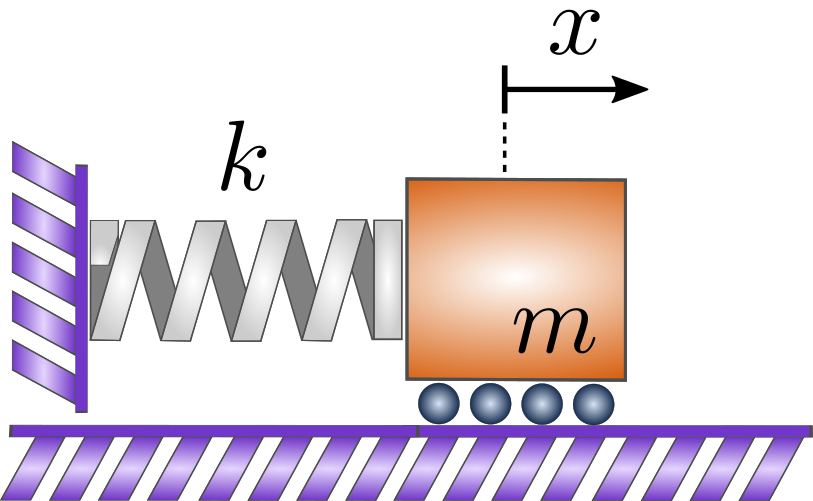
\includegraphics[scale=.17]{fancy_mass_spring.png}
			
		Previously we derived the free response of the mass spring system.
	
		\end{multicols}

		Equation of Motion: \\		
		\[m\ddot{x}+kx=0 \hspace{1mm},\hspc x(0)\hspace{1mm} ,\hspc \dot{x}(0)\] \\
				
		Free Response: \\
		\[ x(t)=Acos\sqrt{\frac{k}{m}}t+Bsin\sqrt{\frac{k}{m}}t \]

	}
	
	% Section I - Frame II
	\frame{ \small
		\frametitle{\sectiontitleI}
	
		\[ x(t)=Acos\sqrt{\frac{k}{m}}t+Bsin\sqrt{\frac{k}{m}}t \] \\
		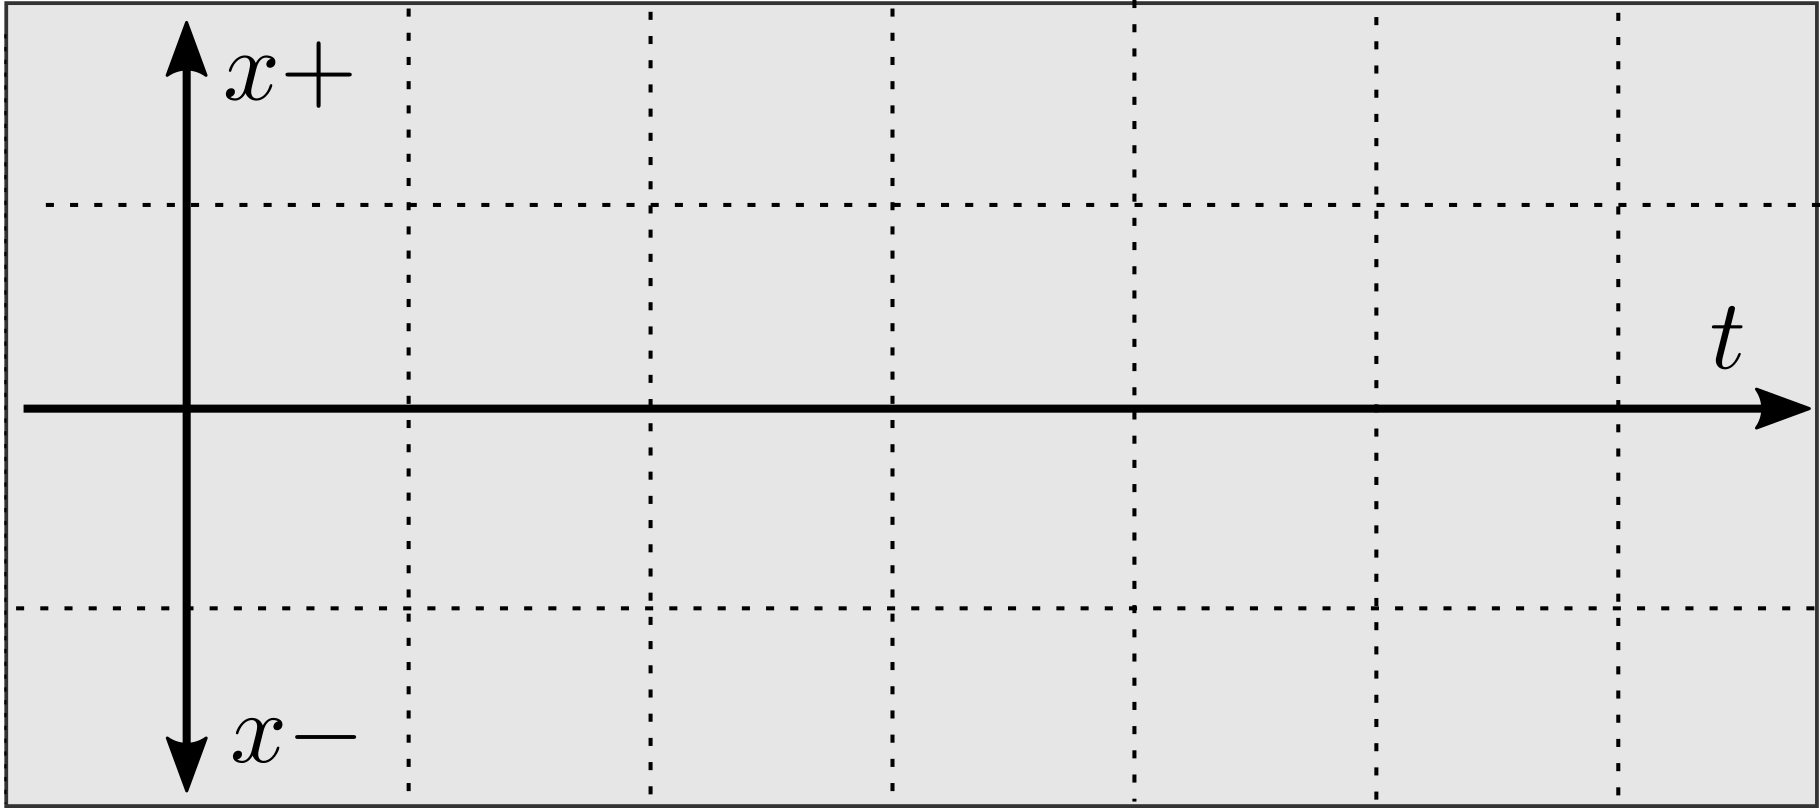
\includegraphics[scale=.18]{time_axis.png} \vspc
	Is this valid? Do you believe it? \vspc
	}

% Section II
\section{\sectiontitleII}
	
	% Section II - Frame I
	\frame{ \small
		\frametitle{\sectiontitleII}
		\[x(t)=e^{\alpha t}\left[ Acos\sqrt{\frac{k}{m}}t+Bsin\sqrt{\frac{k}{m}}t \right]\] \\
		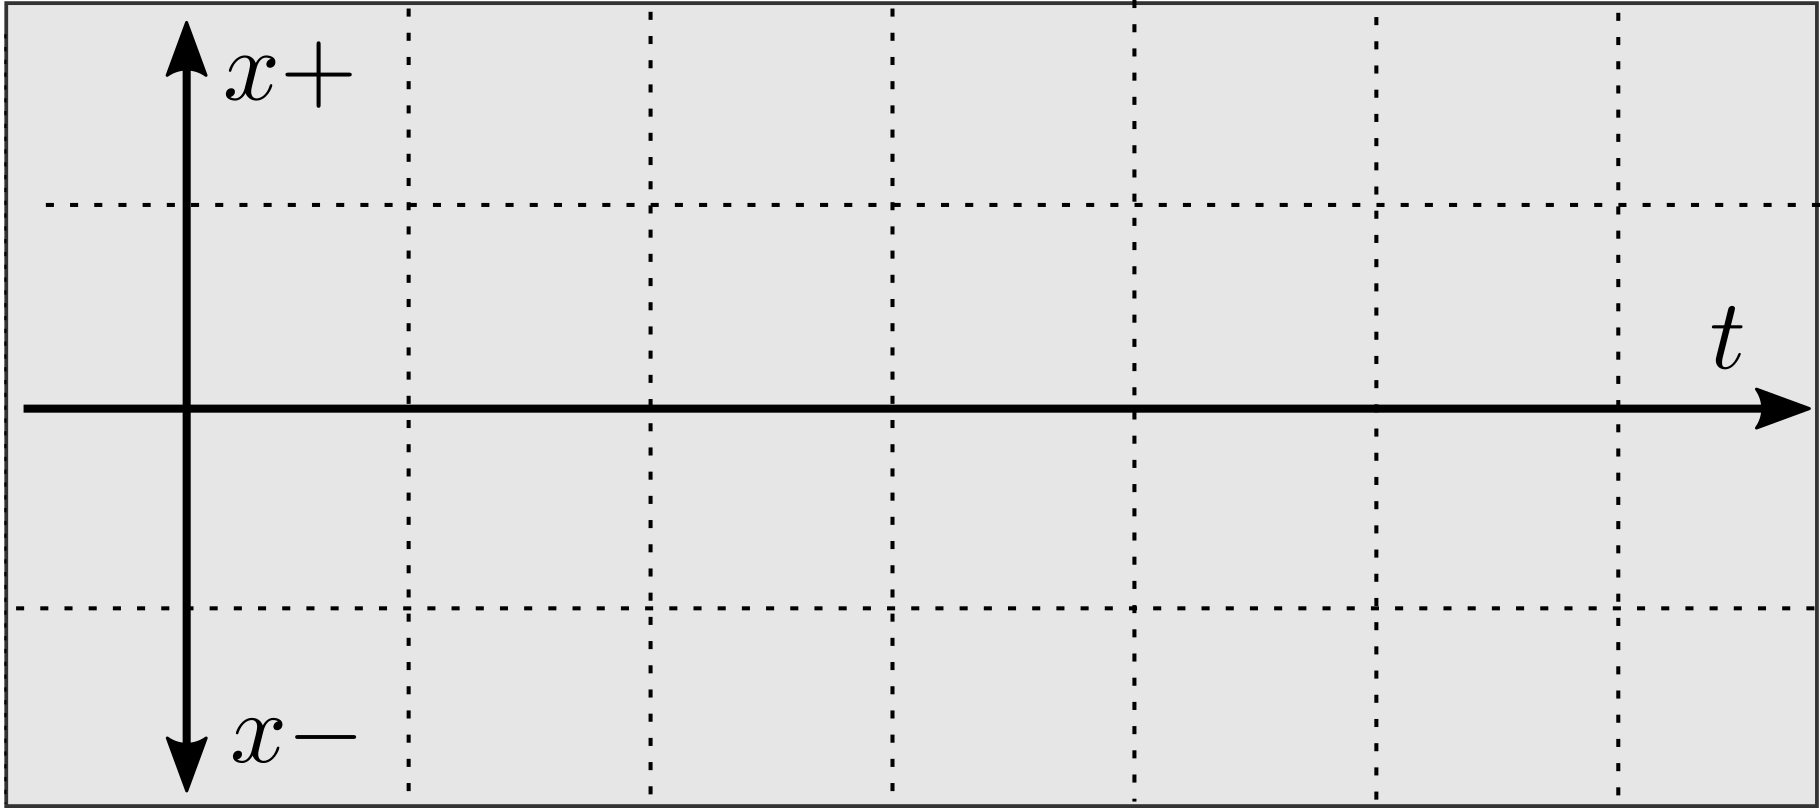
\includegraphics[scale=.18]{time_axis.png} \vspc
		This is much more realistic. \vspc
	}
	
	% Section II - Frame II
	\frame{ 
		\frametitle{\sectiontitleII}
How fast does the system response decay? \vspc What is steady state value?
	
	
	}

% Section III
\section{\sectiontitleIII}
	
	% Section III - Frame I
	\frame{
		\frametitle{\sectiontitleIII}
		
		Damping is a natural phenomenon that cannot be avoided. However in some situations the its influence is significant and in others it is not. \vspc
		\begin{itemize}
			\item		
			\item
		\end{itemize}
		
		The design of many machines depends on the concept of damping and often a mechanical damper is an intentional component of the design.
		 \begin{itemize}
			\item		
			\item
		\end{itemize}

		}
		
% Section IV:
\section{\sectiontitleIV}

	% Section IV - Frame I
	\frame{
		\frametitle{\sectiontitleIV}


	\begin{multicols}{2}

	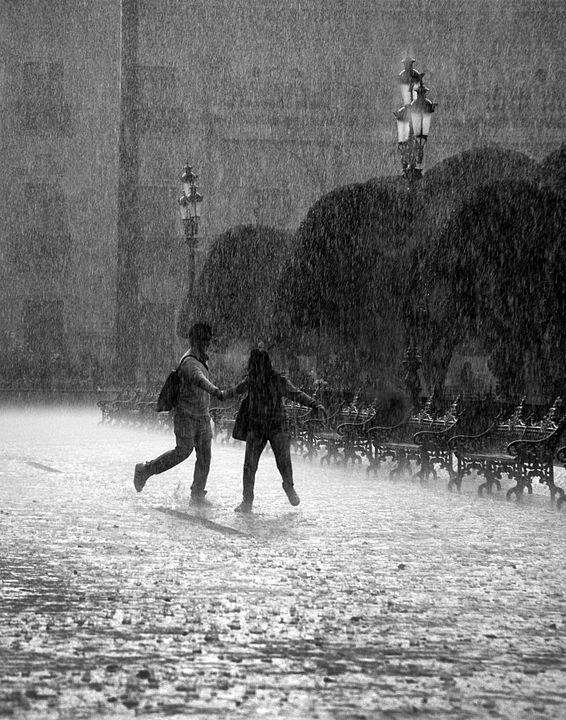
\includegraphics[scale=.20]{rain.jpg}
	
	Dampers Damp!\vspcc
	Rain Dampens...
		
	\end{multicols}
	{\tiny Image: \href{ https://commons.wikimedia.org/w/index.php?curid=19371740}{Wikimedia}}
	

	}
	
\end{document}




